В методах активной балансировки используются различные накопители энергии.
Алгоритм зарядки перенаправляет энергию от перезаряженной ячейке к менее заряженной.
Основные элементы таких схем это конденсаторы, дроссели, трансформаторы. 
Реже используются импульсные dc-dc преобразователи.

\begin{figure}[h]
    \centering
    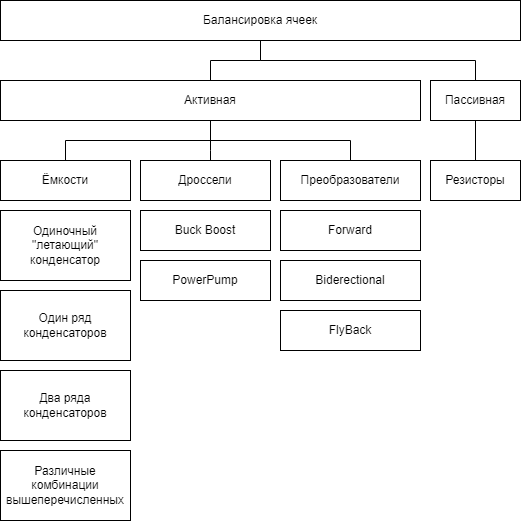
\includegraphics[width=0.6\linewidth]{img/classification.png}
    \caption{Методы балансировки}
    \label{fig:classification}
\end{figure}

\subsubsection{Методы на основе только емкостей}

\subsubsection{Методы на основе только дросселей}

\subsubsection{Метод на основе DC-DC преобразователей}

\subsubsection{Другие методы}